\documentclass[border=10pt]{standalone}
\usepackage{xcolor}
\usepackage{pgf}
\usepackage{tikz}
\usetikzlibrary{arrows.meta}

\usetikzlibrary{arrows}
\usetikzlibrary{calc}
\usetikzlibrary{shapes}
\usetikzlibrary{trees}
\usetikzlibrary{patterns}
\tikzset{>=stealth'}

% for pic 3
\usetikzlibrary{decorations.pathreplacing,calligraphy}

\newcommand{\blue}{\color{blue}}
\newcommand{\black}{\color{black}}

\begin{document}


%pic 3
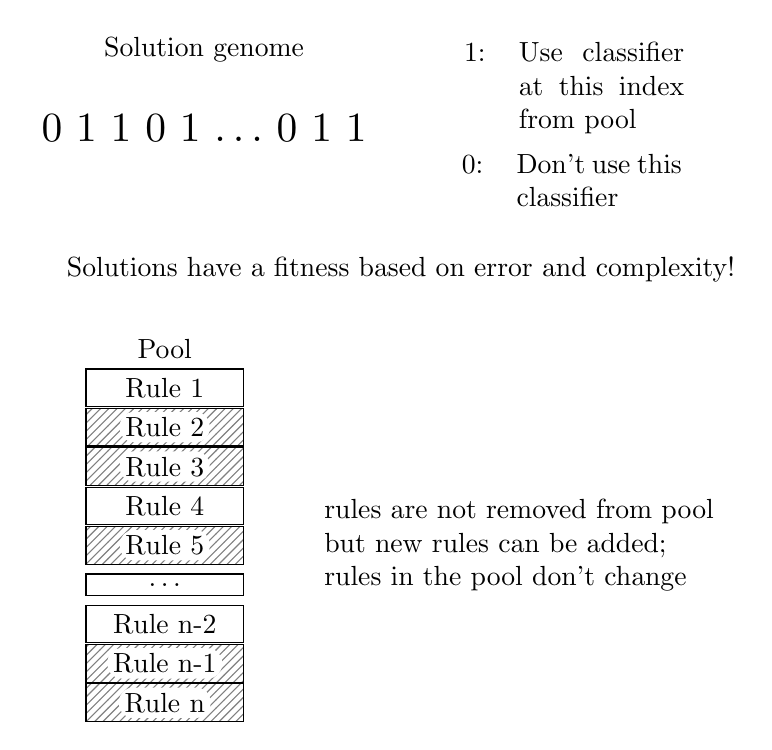
\begin{tikzpicture}[every node/.style={draw=none,minimum width=2cm,align=center}]

\draw node[] (sg) {Solution genome};
\draw node[scale=1.5] at (0,-1) (bin) {0 1 1 0 1 $\ldots$ 0 1 1};
%\draw node at (-1.3,-0.8) (p) {current pool\\ length};
%\draw [decorate,thick,decoration = {calligraphic brace}] (-1.8,0.3) --  (1.8,0.3);
%\draw [decorate,thick,decoration = {calligraphic brace}] (0.5,-0.3) --  (-3,-0.3);

\draw node[right of=sg,xshift=3.7cm,yshift=-.5cm,align=left] (one) {\begin{tabular}{cp{2.1cm}}
1: & Use classifier at this index from pool \\
\end{tabular}};
\draw node[below of=one,xshift=-0.03cm,yshift=-0.2cm,align=left] (zero) {\begin{tabular}{cp{2.1cm}}0: & Don't use this classifier\end{tabular}};

\draw node[below of=bin,xshift=2.5cm,yshift=-.8cm,align=left] (s) {Solutions have a fitness based on error and complexity!};

%\begin{tikzpicture}[every node/.style={draw=none,rectangle,minimum width=1.7cm,minimum height= 0.5cm,align=center}]

\draw node[below of=s,xshift=-3cm] (pool) {Pool};
%\draw node[draw=black,below of=pool,yshift=0.5cm] (cla) {Rule 1};
\draw node[draw=black,yshift=0.5cm,below of=pool] (cla) {Rule 1};
\draw node[draw=black,pattern=north east lines,pattern color=black!50,below of=cla,yshift=0.5cm] (clb) {Rule 2};
\draw node[draw=black,pattern=north east lines,pattern color=black!50,below of=clb,yshift=0.5cm] (clc) {Rule 3};
\draw node[draw=black,below of=clc,yshift=0.5cm] (cld) {Rule 4};
\draw node[draw=black,pattern=north east lines,pattern color=black!50,below of=cld,yshift=0.5cm] (cle) {Rule 5};
\draw node[draw=black,below of=cle,yshift=0.5cm] (clf) {$\ldots$};
\draw node[draw=black,below of=clf,yshift=0.5cm] (clw) {Rule n-2};
\draw node[draw=black,pattern=north east lines,pattern color=black!50,below of=clw,yshift=0.5cm] (clx) {Rule n-1};
%\draw node[draw=black,below of=clx,yshift=0.5cm] (cly) {Rule n};
\draw node[draw=black,pattern=north east lines,pattern color=black!50,below of=clx,yshift=0.5cm] (cly) {Rule n};

\draw node[fill=white,rounded corners=5pt,below of=cla,minimum width=0.5cm,minimum height= 0.2cm,yshift=0.5cm,inner xsep=2pt, inner ysep=2pt] (clb2) {Rule 2};
\draw node[fill=white,rounded corners=5pt,below of=clb,minimum width=0.5cm,minimum height= 0.2cm,yshift=0.5cm,inner xsep=2pt, inner ysep=2pt] (clc2) {Rule 3};
\draw node[fill=white,rounded corners=5pt,below of=cld,minimum width=0.5cm,minimum height= 0.2cm,yshift=0.5cm,inner xsep=2pt, inner ysep=2pt] (cle2) {Rule 5};
\draw node[fill=white,rounded corners=5pt,below of=clw,minimum width=0.5cm,minimum height= 0.2cm,yshift=0.5cm,inner xsep=2pt, inner ysep=2pt] (clx2) {Rule n-1};
\draw node[fill=white,rounded corners=5pt,below of=clx,minimum width=0.5cm,minimum height= 0.2cm,yshift=0.5cm,inner xsep=2pt, inner ysep=2pt] (clx3) {Rule n};


\draw node[right of=clf,xshift=3.5cm,yshift=.5cm,align=left] (rules) {rules are not removed from pool\\ but new rules can be added;\\ rules in the pool don't change};

\end{tikzpicture}



\end{document}

